\chapter{Implementation}
\section{Software architecture}
Continue the IMP tool, all the functions for this task was saved in the \textbf{impls\_2015} package of program. Besides the method was created by myself, I also use some methods from the OpenCV (library for image processing) and Qt framework (framework for C++).\\[0.2cm]
\begin{figure}[h!]
\centering
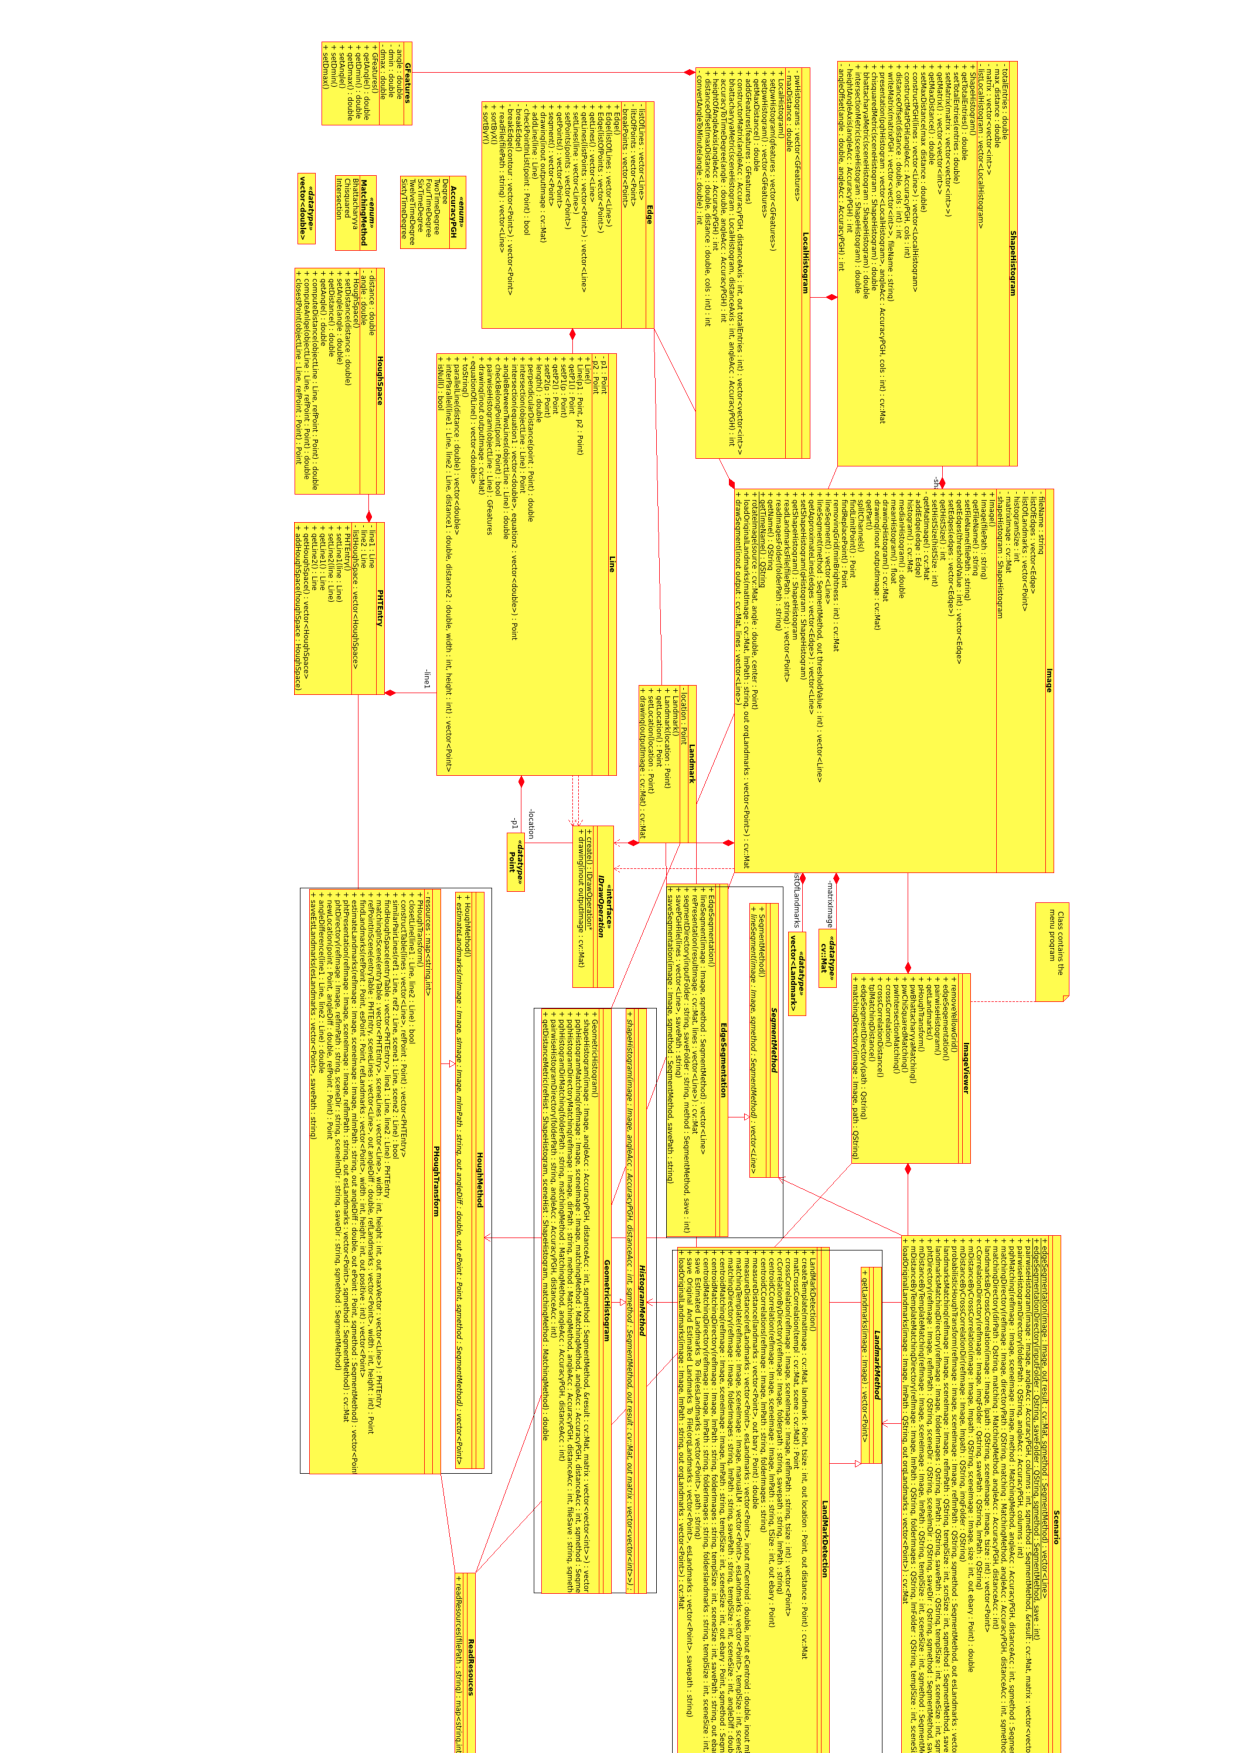
\includegraphics[width=0.9\textwidth]{images/cdiagram}
\caption{The class diagram of program}
\label{fig:cdiagram}
\end{figure}
The class diagram\footnote{See the full image in Appendix} in \ref{fig:cdiagram} show mainly classes of my task. The \textit{mainly} methods located in the \textit{ImageViewer} class, where contains all functions of the software. To represent the information of image and preprocessing about clear the yellow grid, we use the classes such as \textit{Line}, \textit{Edge}, \textit{Landmark}, \textit{YellowGird}, \textit{Image} class. For the edge segmentation, construct the geometric histogram and landmarks detection, we have \textit{GFeatures}, \textit{LocalHistogram}, \textit{ShapeHistogram}, \textit{EdgeSegmentation}, \textit{LandmarkDection} class. All the main functions were inherated from the \textit{IExtraction} interface and used in \textit{main} class via the \textit{Sceneario} class. The aim, properties and methods in each class was discussed in below sections.
\section{Image preprocessing}
The \textit{Image processing} section contains the information about the classes which describe the geometric objects can be represent the image and the method to remove the yellow grid on the images.
\subsection{Line class}
\textbf{Line} class describe the information of a straight line and the methods can do with a line.
\subsubsection{The attributes}
\begin{itemize}
\item\textbf{p1}: the first endpoint of line.
\item\textbf{p2}: the second endpoint of line.
\end{itemize}
\subsubsection{The methods}
\begin{itemize}
\item\textbf{Line()}: Constructor an empty line.
\item\textbf{Line(p1: Point, p2: Point)}: Constructor a line with two endpoints p1, p2. With type of the endpoints is \textbf{Point} (in OpenCV)
\item\textbf{getP1()}: Getter the first endpoint 
\item\textbf{setP1(p:Point)}: Setter the first endpoint
\item\textbf{getP2()}: Getter the second endpoint 
\item\textbf{setP2(p:Point)}: Setter the second endpoint
\item\textbf{length()}: Calculate the length of line
\item\textbf{perpendicularDistance(point:Point)}: Compute the perpendicular distance from point ``\textbf{point}" to the line
\item\textbf{angleBetweenTwoLines(objectLine: Line)}: Compute the angle between two lines.
\item\textbf{checkBelongPoint(point: Point)}: Check a point stay on the line or not. If the point stay on the line, the return value is true; otherwise, return false.
\item\textbf{intersection(objectLine: Line)}: Finding the intersection point of two lines. If two lines have intersect, the method will return the coordinate of intersection point; otherwise, method will return a negative point.
\item\textbf{interection(equation1:vector<double>, equation2: vector<doube>)}: Finding the intersection of two lines. In this case, the lines presented under $y=ax + b$, and vector input contains three coefficient of line.
\item\textbf{pairwiseHistogram(objectLine: Line)}: Finding the geometric features between two lines. The return value is an \textbf{GFeatures} object, it includes the information of angle between two lines, the distance from two endpoints of \textit{objectLine} to the reference line.
\item\textbf{equationOfLine()}: Calculate the equation of line. 
\item\textbf{drawing(outputImage: Mat)}: Drawing the line on the output image.
\item\textbf{operator==(line:Line)}: Defining the equal lines.
\item\textbf{parallelLine(distance: double)}: Finding the lines parallel with it and the distance between them is $distance$. If found, the method return a list of equation of the lines.
\item\textbf{interParallel(line1: Line, line2: Line, distance1: double, distance2: double, width: int, height: int)}: Finding the intersection between two lines parallel with $line1$ and $line2$ in an image have the size $width x height$. The distance from $line1$ to its parallel line is $distance1$, the distance between $line2$ and its parallel is $distance2$.
\item\textbf{isNull()}: Checking a line is null. Method return $true$ if two endpoints of line are equal, otherwise return $false$.
\end{itemize}
\subsection{Edge class}
The \textbf{Edge} class used to presented for a curve and the methods with edge. An edge can be presented by a list of lines or a list of points.
\subsubsection{The attributes}
\begin{itemize}
\item\textbf{listOfLines}: list of approximate lines of edge.
\item\textbf{listOfPoints}: list of point represented edge.
\item\textbf{breakPoints}: list of break points on edge when edge broken to the approximate lines.
\end{itemize}
\subsection{The methods}
\begin{itemize}
\item\textbf{Edge()}: Construct an empty edge.
\item\textbf{Edge(lines: vector\textless Line\textgreater)}: Constructor an edge from a list of lines.
\item\textbf{Edge(point: vector\textless Point\textgreater)}: Constructor an edge from a list of points.
\item\textbf{getLines()}: Get the lines of edge.
\item\textbf{getLines(listPoints: vector\textless Point\textgreater)}: Get the lines from a list of points.
\item\textbf{setLines(lines: vector\textless Line \textgreater)}: Set the lines of edge.
\item\textbf{getPoints()}: Get the points of edge.
\item\textbf{addLine(line: Line)}: Add a line into the list of lines of edge.
\item\textbf{readFile(filePath: QString)}: Get the list lines of edge from a file.
\item\textbf{breakEdge(),segment()}: Break edge into approximate lines from the list points of edge.
\item\textbf{drawing(outputImage Mat)}: Draw edge
\end{itemize}
\subsection{Image class}
\textbf{Image} class presented the information of an image such as file name, list of edge extracted from it,... and the methods with image.
\subsubsection{The attributes}
\begin{itemize}
\item\textbf{fileName}: File name of image
\item\textbf{listOfEdges}: List of edges extracted from image
\item\textbf{listOfLandmarks}: List of landmark of image
\item\textbf{matrixImage}: Matrix represented for image
\item\textbf{pghHistogram}: Pairwise geometric histogram (PGH) presented for image
\item\textbf{histogramSize}: Histogram size of image (256)
\end{itemize}
\subsubsection{The methods}
\begin{itemize}
\item\textbf{Image()}: Construct an empty image
\item\textbf{Image(filePath: QString)}: Construct an image with a full path
\item\textbf{getFileName()}: Get the full path of image
\item\textbf{setFileName(filePath: QString)}: Set the path of image
\item\textbf{getEdges()}: Get the edges from image
\item\textbf{setEdges(edges: vector \textless Edge\textgreater)}: Set the edges of image
\item\textbf{getMatrixImage()}: Get the matrix presentation of image
\item\textbf{addEdge(edge: Edge)}: Add an edge into list edges of image
\item\textbf{histogram()}: Get the histogram of image
\item\textbf{medianHistogram()}: Compute the median of histogram of image
\item\textbf{meanHistogram()}: Compute the mean of histogram of image
\item\textbf{drawingHistogram()}: Draw the histogram of image
\item\textbf{drawing(outputImage: Mat)}: Draw image
\item\textbf{getPart()}: Get the kind of image (elytre, tete, mandibule,...)
\item\textbf{splitChannels()}:  Split the image into several channel colors, if image in BGR mode.
\item\textbf{findLimitPoint()}: Find the ``limit point" of yellow grid
\item\textbf{findReplacePoint()}: Find the ``replace point"
\item\textbf{removingGrid(minBrightness: int)}: Remove the yellow grid on image
\item\textbf{lineSegment()}: Segment the edges of image into set of approximate lines.
\item\textbf{setShapeHistogram(shapeHist: ShapeHistogram)}: Set PGH of image.
\item\textbf{getShapeHistogram()}: Get PGH histogram of image
\item\textbf{readLandmarksFile(filePath: string)}: Read the landmarks of image from a file
\item\textbf{readFolder(folderPath: QString)}: Read the images from a folder.
\item\textbf{getName()}: Get name only of image.
\end{itemize}
\section{Automatic classification }
about methods
\section{Result}
result...





























